%!TEX root = ../talk.tex

\section{TensorFlow}\label{sec:TF}

%%%
\subsection{Computational graph}
%%%

\begin{frame}[fragile]
  \MyLogo
  \frametitle{Computational graph}  
TensorFlow computations are expressed as stateful dataflow graphs.
\begin{itemize}
\item each node corresponds to an operation (eg tensor, add, sub etc)
\item each edge corresponds to tensor flowing direction
\end{itemize}
%  
\begin{columns}
\column{.57\textwidth}
\begin{lstlisting}[language=python]
node1 = tf.constant(3.0, tf.float32)
node2 = tf.constant(4.0)
node3 = tf.add(node1, node2)
add_and_triple = adder_node * 3
\end{lstlisting}
%
\column{.48\textwidth}
%
\begin{figure}[htbp] 
   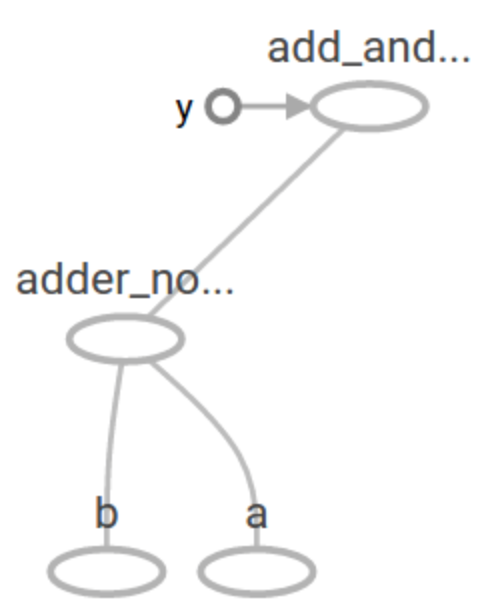
\includegraphics[height=1.5in]{figures/compgraph.png} 
\caption{Computaion graph}
\end{figure}
\end{columns}
\end{frame}

%%%
\subsection{Programming interface}
%%%

\begin{frame}
  \MyLogo
  \frametitle{Programming interface}  

\end{frame}

%%%
\subsection{Visualization}
%%%

\begin{frame}
  \MyLogo
  \frametitle{Visualization: TensorBoard}  

\begin{columns}
\column{.48\textwidth}  
\scriptsize{
Computation graphs are powerful but complicated
\begin{itemize}
\item  thousands of nodes or more 
\item  network is deep
\item  graph visualization tool TensorBoard is helpful
\end{itemize}
}
%
\column{.5\textwidth}
\begin{figure}[htbp] 
   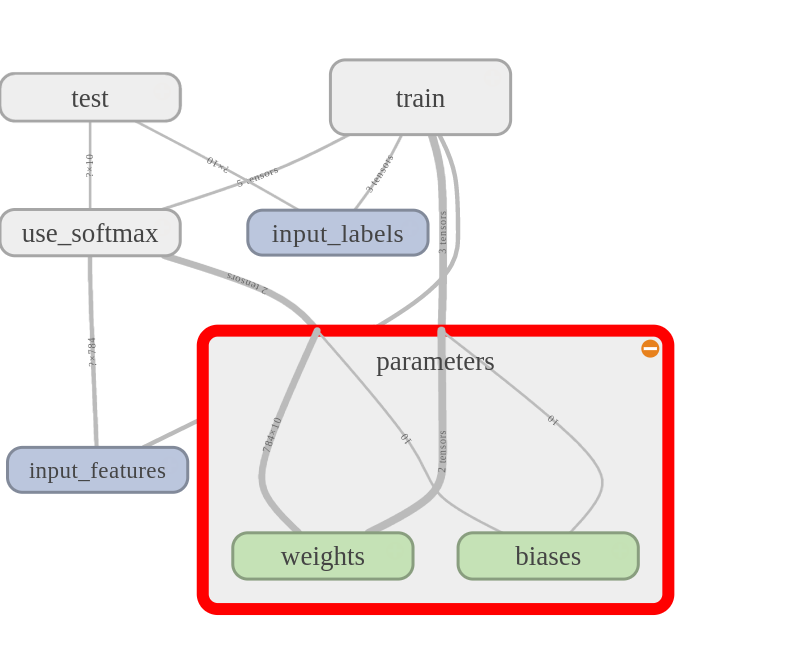
\includegraphics[height=2.5in]{figures/graphvisualization.png} 
\caption{Graph Visualization}
\end{figure}
\end{columns}

\end{frame}

%%%
\subsection{Some examples}
%%%

\begin{frame}[fragile]
  \MyLogo
  \frametitle{Example 1: SoftMax}  
 
\scriptsize{
\begin{lstlisting}[language=python]
import tensorflow as tf    

X = tf.placeholder(tf.float32, [None, 28, 28, 1])     
W = tf.Variable(tf.zeros([784, 10]))    
b = tf.Variable(tf.zeros([10]))   
init = tf.initialize_all_variables() 

# model
Y= tf.nn.softmax(tf.matmul(tf.reshape(X,[-1, 784]), W) + b)  

# placeholder for correct answers    
Y_ = tf.placeholder(tf.float32, [None, 10])  

# loss function   
cross_entropy = -tf.reduce_sum(Y_ * tf.log(Y))  

# % of correct answers found in batch
is_correct = tf.equal(tf.argmax(Y,1), tf.argmax(Y_,1))  
accuracy = tf.reduce_mean(tf.cast(is_correct,tf.float32))  
\end{lstlisting}
}
\end{frame}

\begin{frame}[fragile]
  \MyLogo
  \frametitle{Example 1:SoftMax}  
 
\scriptsize{
\begin{lstlisting}[language=python]
optimizer = tf.train.GradientDescentOptimizer(0.003)
train_step = optimizer.minimize(cross_entropy)

sess = tf.Session()
sess.run(init)

for i in range(10000):
	# load batch of images and correct answers
	batch_X, batch_Y = mnist.train.next_batch(100)
       	train_data={X: batch_X, Y_: batch_Y}

	# train
	sess.run(train_step, feed_dict=train_data)

	# success ? add code to print it
	a,c = sess.run([accuracy, cross_entropy], feed=train_data)

	# success on test data ?
	test_data={X:mnist.test.images, Y_:mnist.test.labels}
	a,c = sess.run([accuracy, cross_entropy], feed=test_data)
\end{lstlisting}
}

%\end{tabular}

%\end{center}
%\label{default}
%\end{table}%
\end{frame}